\section{Architektur- und UI-Design}
\label{sec:Design}

\subsection{UMLv1 - 30.11.2015}
\begin{figure}[h]
\caption{UMLv1}
\centering
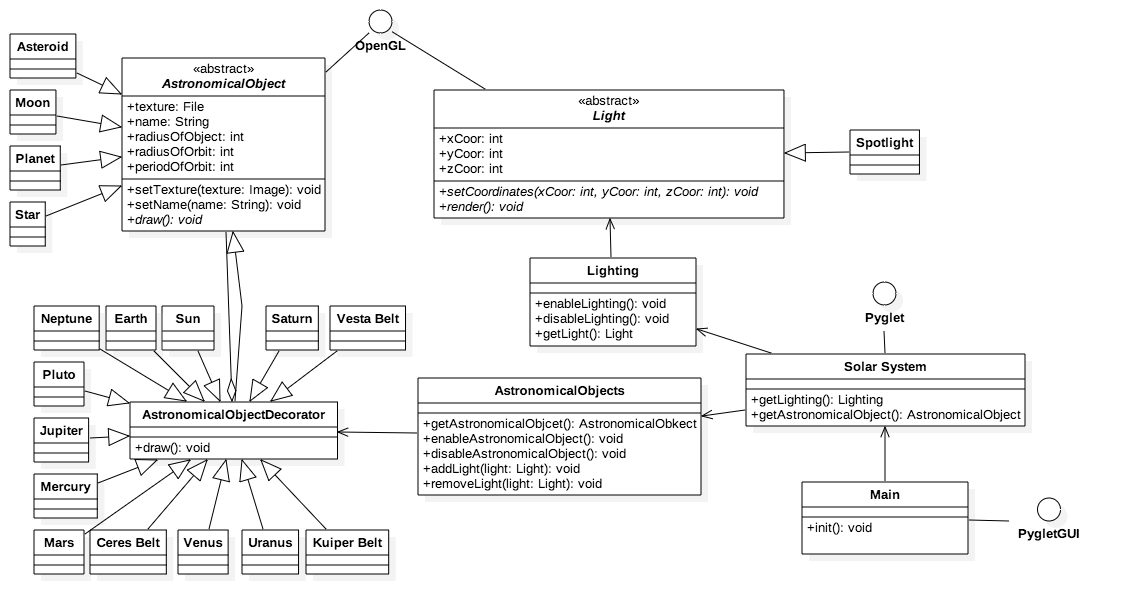
\includegraphics[scale=0.4]{images/UML-30112015_v1.png}
\end{figure}

Im ersten UML wurde wert auf verwnedung von Design-Patterns, Einbindung der benötigten Interfaces und Libraries, und grobe
veranschaulichung der Architektur gelegt. Glücklicherweise war dieser erste Ansatz auch ein sehr guter bei welchem nur 
Kleinigkeiten geändert wurden (siehe v2). Wie man erkennen kann wird das Decorator und Abstract Factory Pattern verwendet. 

\clearpage
\subsection{UMLv2 - 15.12.2015}
\begin{figure}[h]
\caption{UMLv2}
\centering
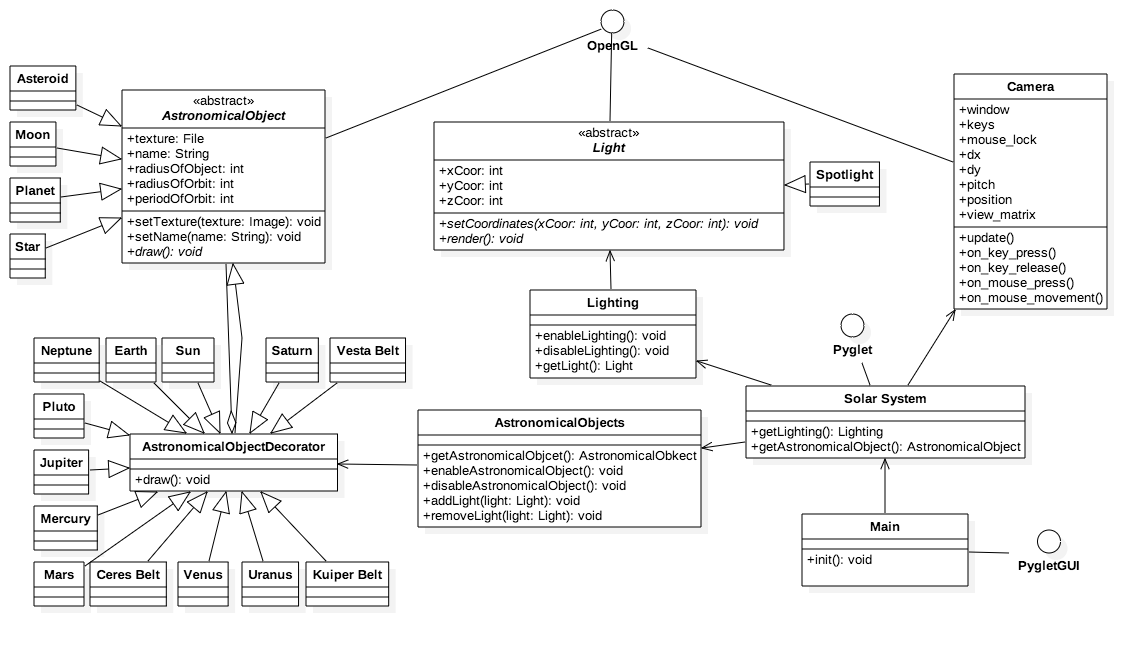
\includegraphics[scale=0.4]{images/UML-15122015_v2.png}
\end{figure}
Wie bereits erwähnt musste nur relativ wenig vom ersten Design geändert werden. Wir haben hier eine eigene Klasse für
die Kamera entwickelt. Mann muss dazu sagen, es sollte eigentlich eine v3 auch geben, da wir einige andere Module
ebenfalls hinzugefügt haben.

\clearpage
\subsection{GUI-Konzept}
Folgendes GUI-Konzept wurde umgesetzt.

\begin{figure}[h]
\centering
\begin{minipage}{.5\textwidth}
  \centering
  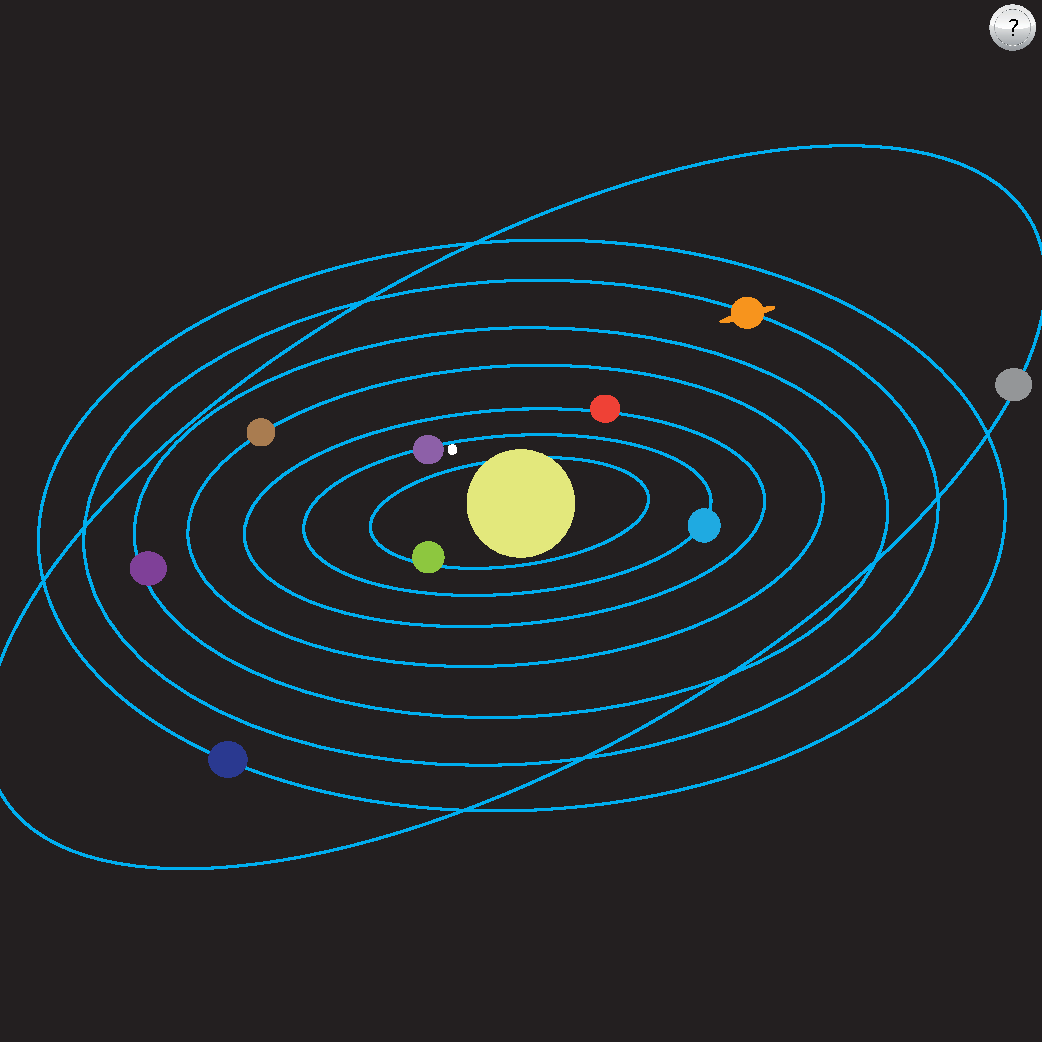
\includegraphics[scale=0.4]{images/GUI-Concept_Planets_side.pdf}
  \captionof{figure}{GUI-Concept: Planets from side}
  \label{fig:test1}
\end{minipage}%
\begin{minipage}{.5\textwidth}
  \centering
  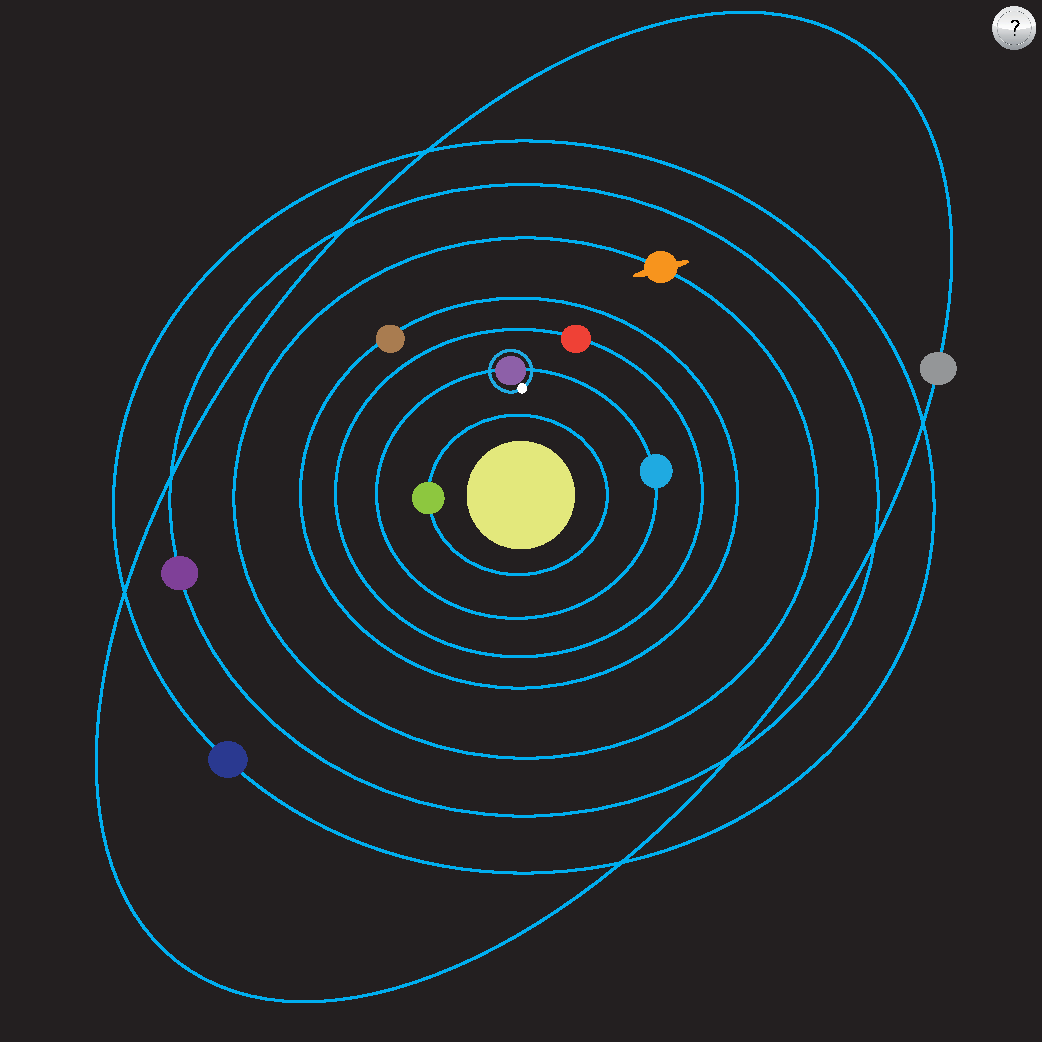
\includegraphics[scale=0.4]{images/GUI-Concept_Planets_top.pdf}
  \captionof{figure}{GUI-Concepts: Planets from top}
  \label{fig:test2}
\end{minipage}
\end{figure}

\begin{figure}[h]
\centering
\includegraphics[scale=0.4]{images/GUI-Concept_Startscreen.pdf}
\caption{GUI-Concept: Startscreen}
\end{figure}

